\documentclass{article}
\usepackage{amsmath}
\usepackage{amsfonts}
\usepackage{graphicx}
\usepackage{listings}
\usepackage{color} %red, green, blue, yellow, cyan, magenta, black, white

\definecolor{codegreen}{rgb}{0,0.6,0}
\definecolor{codegray}{rgb}{0.5,0.5,0.5}
\definecolor{codepurple}{rgb}{0.58,0,0.82}
\definecolor{backcolour}{rgb}{0.95,0.95,0.92}

 
\title{Machine Learning lecture notes}
\author{Khoa Hoang Viet \thanks{based on Andrew Ng's Machine Learning course in coursera.org}}
\date{\today}
\begin{document}
\section{Evaluating a Learning Algorithm}
\subsection{Deciding What to Try Next}
There's often a huge difference between someone that really knows how to powerfully and effectively apply that algorithm, versus someone that's less familiar with some  doesn't really understand how to apply these algorithms and can end up wasting a lot of their time trying things out that don't really make sense.

Practical suggestions, advice, guidelines on how to choose one of the most promising avenues to spend your time pursuing when developing machine learning systems.

There are many things that one can think of that could improve the performance of the learning algorithm:
\begin{itemize}
	\item Get more training examples( But sometimes getting more training data doesn't actually help )
	\item Try a smaller set of features
	\item Get additional features
	\item Adding polynomial features things
	\item Increase or decrease the regularization: $\lambda$
\end{itemize}

We need \textbf{evaluate learning algorithms} to rule out half of the things on this list as being potentially promising things to pursue. The techniques are called \textbf{Machine learning diagnostics.}

Machine learning diagnostics: A test that you can run to gain insight what is/isn’t working with a learning algorithm, and gain guidance as to how best to improve its performance

\subsection{Evaluating a hypothesis}
\subsubsection{How?}
Split the data we have into two portions: The first portion is going to be our usual \textbf{training set} and the second portion is going to be our \textbf{test set}

m: denote number of training dataset (70\%)

$m_{test}$: denote number of testset (30\%)

\noindent The new procedure using these two sets is then:

\begin{enumerate}
	\item Learn $\Theta$ and minimize $J_{train}(\Theta)$ using the training set
	\item Compute the test set error $J_{test}(\Theta)$
\end{enumerate}

\subsubsection{The test set error}
For linear regression: $J_{test}(\Theta) = \dfrac{1}{2m_{test}} \sum_{i=1}^{m_{test}}(h_\Theta(x^{(i)}_{test}) - y^{(i)}_{test})^2$

For classification ~ Misclassification error (aka 0/1 misclassification error):
$$err(h_\Theta(x),y) = \begin{matrix} 1 & \mbox{if } h_\Theta(x) \geq 0.5\ and\ y = 0\ or\ h_\Theta(x) < 0.5\ and\ y = 1\\ 0 & \mbox otherwise \end{matrix}$$

This gives us a binary 0 or 1 error result based on a misclassification. The average test error for the test set is:
$$\text{Test Error} = \dfrac{1}{m_{test}} \sum^{m_{test}}_{i=1} err(h_\Theta(x^{(i)}_{test}), y^{(i)}_{test})$$

This gives us the proportion of the test data that was misclassified.

\section{Handling Skewed Data}
\textbf{Skewed Data} is data has asymmetrical distribution. Example: In cancer classification that just 1\% of patients have cancer.
In that case, use accuracy metric as evalution metric seem like not good at all. 
\subsection{Error Metrics for Skewed Data}
First we split the outcome value to 4 classes:

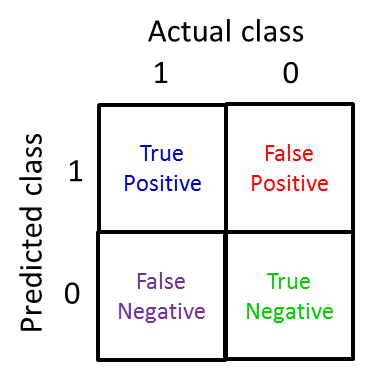
\includegraphics[width=\textwidth]{TP_FP_TN_FN.png}

With these classes we can here is how to caculate \textbf{Precision/Recall} metrics:
$$\textbf{Precision} = \frac{\text{True positives}}{\text{\# predicted as positive}} = \frac{\text{True positives}}{\text{True positives + False positives}}$$

$$\textbf{Recall} = \frac{\text{True positives}}{\text{\# actual positives}} = \frac{\text{True positives}}{\text{True positives + False negatives}}$$


Note: y=1 small class(e.g: cancer patients), y=0 for larger class(e.g:non-cancer patients).

\end{document}